\documentclass[11pt,a4paper]{report}
\setcounter{secnumdepth}{3} % default is 2
\usepackage{amsmath, amsfonts, amssymb, amsthm}
\usepackage{graphicx}
\graphicspath{ {img/} }
\usepackage{xspace}
\usepackage{color}
\usepackage{array}
\usepackage{booktabs}
\usepackage{enumitem}
\usepackage{multirow}
\usepackage{listings}
\usepackage[colorlinks=true,citecolor=blue,linkcolor=blue,urlcolor=blue]{hyperref}
\usepackage{a4wide}
\usepackage{subcaption}
\usepackage[utf8]{inputenc}
\usepackage[noline]{algorithm2e}
\usepackage{siunitx}

\usepackage{tikz}
\usepackage{pgfplots}
\pgfplotsset{compat=1.9}

%\usepackage[sc]{mathpazo}
\usepackage[default,osfigures,scale=0.95]{opensans}
\renewcommand*\familydefault{\sfdefault}
\usepackage[T1]{fontenc}

\usepackage{cmbright}
\SetSymbolFont{largesymbols}{normal}{OMX}{iwona}{m}{n}


\usepackage{titlesec}
\titleformat{\chapter}
  {\normalfont\LARGE\bfseries}{\thechapter}{1em}{}
  \titlespacing*{\chapter}{0pt}{3.5ex plus 1ex minus .2ex}{2.3ex plus
  .2ex}

\usepackage[nottoc]{tocbibind}
\usepackage{microtype}
\usepackage{mathtools}

\usepackage[capitalize]{cleveref}

\crefformat{section}{\S#2#1#3}
\crefmultiformat{section}{\S\S#2#1#3}{ and~#2#1#3}{, #2#1#3}{, and~#2#1#3}

\hfuzz=3pt
\setlength\parindent{0pt}
\setlength{\parskip}{1em}
\setcounter{tocdepth}{2}

\definecolor{green}{RGB}{0,140,0}
\definecolor{blue}{RGB}{0,89,153}
\definecolor{yellow}{RGB}{250,150,0}
\definecolor{red}{RGB}{255,76,25}

% predefined LaTeX colors
\newcommand{\tcg}[1]{\textcolor{green}{#1}}
\newcommand{\tcb}[1]{\textcolor{blue}{#1}}
\newcommand{\tcr}[1]{\textcolor{red}{#1}}
\newcommand{\tcy}[1]{\textcolor{yellow}{#1}}

\definecolor{GREEN}{RGB}{204,235,204}
\definecolor{BLUE}{RGB}{178,201,232}
\definecolor{RED}{RGB}{232,178,178}
\definecolor{YELLOW}{RGB}{255,252,204}

\newcommand{\tcng}[1]{\textcolor{GREEN}{#1}}
\newcommand{\tcnb}[1]{\textcolor{BLUE}{#1}}
\newcommand{\tcnr}[1]{\textcolor{RED}{#1}}
\newcommand{\tcny}[1]{\textcolor{YELLOW}{#1}}


% abbreviations
\newcommand\NOT {\texttt{NOT}\xspace}
\newcommand\OR {\texttt{OR}\xspace}
\newcommand\AND {\texttt{AND}\xspace}
\newcommand\XOR {\texttt{XOR}\xspace}
\newcommand\NAND {\texttt{NAND}\xspace}
\newcommand\NOR {\texttt{NOR}\xspace}
\newcommand\TODO{\textbf{TODO}\xspace}

\newcommand{\gravity}{\ensuremath{\textsf{PRUNE-HORST}}\xspace}
\newcommand{\hashx}{\ensuremath{\textsf{Hash}}\xspace}
\newcommand{\hashy}{\ensuremath{\textsf{Hash32}}\xspace}
\newcommand{\hashz}{\ensuremath{\textsf{Hash64}}\xspace}
\newcommand{\drbg}{AES-256-CTR\xspace}
\newcommand{\sk}{\ensuremath{\mathsf{sk}}\xspace}
\newcommand{\ek}{\ensuremath{\mathsf{ek}}\xspace}
\newcommand{\pk}{\ensuremath{\mathsf{pk}}\xspace}
\newcommand{\sig}{\ensuremath{\mathsf{sig}}\xspace}

\newcommand{\hex}[1]{\texttt{#1}}
\newcommand{\xhex}[1]{\scalebox{0.75}{\texttt{#1}}}

\newcommand{\NN}{\ensuremath{\mathbb{N}}}
\newcommand{\FF}{\ensuremath{\mathbb{F}}}

\newcolumntype{C}[1]{>{\centering\let\newline\\\arraybackslash\hspace{0pt}}m{#1}}


\theoremstyle{definition}
\newtheorem{definition}{Definition}
\theoremstyle{plain}
\newtheorem{lemma}{Lemma}
\newtheorem{assumption}{Assumption}
\newtheorem{claim}{Claim}
\theoremstyle{remark}
\newtheorem{remark}{Remark}


% Global algorithm2e configs
\DontPrintSemicolon
\SetArgSty{rmfamily}
\SetNlSty{rmfamily}{}{.}
\SetKwFor{For}{\nl for}{do}{\nl end}
\SetKwIF{If}{ElseIf}{Else}{\nl if}{then}{\nl elif}{\nl else}{\nl end}%
\SetKw{Input}{Inputs:}
\SetKw{Output}{Outputs:}
\SetKw{Algorithm}{Algorithm:}


\begin{document}


\title{
\Huge{\gravity} \\[0.15cm]
\large{v1}, \today
}

\author{
\textbf{Inventor, submitter, main contact:}  \\[0.15cm]
Jean-Philippe Aumasson, Kudelski Security \\[0.15cm]
Route de Genève 22, 1033 Cheseaux-sur-Lausanne, Switzerland \\[0.15cm]
\texttt{jeanphilippe.aumasson@gmail.com}, +41 79 726 05 08 \\[0.5cm]
\textbf{Inventor, submitter, backup contact:}  \\[0.15cm]
Guillaume Endignoux \\[0.15cm]
\texttt{guillaume.endignoux@m4x.org} \\[0.5cm]
}

\date{}

\maketitle



\tableofcontents
\newpage

\chapter{Introduction}\label{chap:introduction}

\gravity is a hash-based \emph{few-time signature scheme}, meaning that it's only secure for a limited number of messages---a dozen, hundreds, or thousands, depending on the version.

This limitation allows \gravity to be relatively simple and efficient. It's also \emph{stateless}, as required by NIST.

\gravity is based on Hash to Obtain Random Subset, or HORS, a stateless few-time signature scheme proposed by Reyzin and Reyzin in 2002~\cite{hors}. Like HORST---a variant of HORS introduced for the SPHINCS construction by Bernstein et al. in 2015~\cite{sphincs}---\gravity reduces HORS' public key size thanks to a Merkle tree. The prefix \textsf{PRUNE} summarizes additional tricks to optimize HORS' security and efficiency:
\begin{itemize}
\item A \emph{pseudo-random} generator is used rather than just a hash function in order to obtain a random subset of a set of integers.
\item The pseudo-random generator allows to ensure that the subset elements are \emph{unique}, which increases the security of the scheme (see~\cite[\S4]{masters} and~\cite{subsetres}
\item The Merkle tree is \emph{pruned} in order to trade signature size for public key size, by eliminating redundant key nodes, similarly to what SPHINCS does to minimize the signature size.
\end{itemize}

\section{Advantages and Limitations}

Advantages:
\begin{itemize}

\item \textbf{Simple}: \gravity is much simpler than hash-based signature schemes such as SPHINCS or XMSS, and than signatures schemes from other post-quantum families. The logic of the scheme fits in about 200 lines of C code.

\item \textbf{High-assurance}: Security essentially depends on the collision resistance of hash functions, an assumption unlikely to fail for the proposed functions. \gravity also leverages our detailed analysis and bounds detailed in~\cite[\S4]{masters} and~\cite{subsetres}.

\item \textbf{Speed/security trade-offs} are easily done by varying the parameters $T$ and $K$. For a given choice of $T$ and $K$, an additional parameter $C$ allows to reduce the signature size at the cost of a larger public key.

\item \textbf{Forgeries detection}: If the limit of messages to be signed is exceeded, thereby making forgeries easier, the legitimate signer can detect such forgeries. Obviously, a signature forged by stealing the secret key couldn't be detected.

\item \textbf{Almost optimal}: the signature size can be further reduced by eliminating redundancies, as is our recent Octopus technique~\cite[\S5]{masters}, however by default \gravity avoids the extra complexity and uses suboptimal-length signatures.

\end{itemize}

Limitations:

\begin{itemize}

\item \textbf{Few-time}: Only a limited number of messages can be signed while retaining the highest security guarantees: about 100 or about 1000, depending on the instance. If more messages than the limit are signed, then security slowly degrades.

\item \textbf{Signature size}: Signatures aren't small, but they can be made smaller by using larger public keys. This trade-off has no security impact, and makes signing faster as the public key size grows.

\end{itemize}


\section{Motivations}

A few-time signature scheme allowing only for hundreds or thousands of
distinct messages to be signed is sufficient in a number of major
applications, such as:
root CAs signing intermediate CA certificates; signing of firmware or bootloader images for long-lived devices; protocols using ephemeral signing keys (as mpOTR did); identify management for device provisioning, for example in messaging applications.

Another class of application would use few-time signatures to enforce a bound in the number of authorized signatures.
For example, a bank might issue a digital checkbook limited to 100 transactions.
Would a client issues more than the authorized 100 signatures, they would reduce their own security and thereby allow an attacker to forge signatures on their behalf.


We chose HORS(T) as a basis because it's the most efficient few-time signature construction, and because of its simplicity.

Primitives in \gravity are SHA-256, AES-256-CTR, and Haraka\,v2~\cite{haraka}.
The latter is not a NIST standard, because we needed a fast, short-input hash function and NIST doesn't provide such a primitive.
Haraka\,v2 hashes 32- or 64-byte input values and produces a 32-byte hash value.
It is based on the AES round function and optimized implementations use AES-NIs.
We chose Haraka\,v2 with 6 rounds, rather than the default 5 round, for a greater assurance against collisions.
\chapter{Specification}\label{chap:specification}

Below ``$\log$'' means ``$\log_2$'', ``$\Vert$'' is string concatenation, all hash values are 32-byte. The type of tree used is a complete binary hash tree (i.e., a complete Merkle tree).

\section{Primitives}

\gravity requires three hash functions, which all return 32-byte hash
values:

\begin{itemize}

\item \hashx takes input values of any length. We use \textbf{SHA-256} as \hashx.

\item \hashy takes input values of 32 bytes. We use \textbf{Haraka-256} with 6 rounds as \hashy.

\item \hashz takes input values of 64 bytes. We use \textbf{Haraka-512} with 6 rounds as \hashz.

\end{itemize}
The Haraka versions are the v2~\cite{haraka}.

\gravity also uses \textbf{AES-256-CTR} as a deterministic generator of pseudorandom bytes.



\section{Parameters}

\gravity signature schemes are defined by three parameters:

\begin{itemize}

\item The \textbf{set size} $T$, which must be a power of two.

\item The \textbf{subset size} $K$, which must be lower than $T$.

\item The \textbf{number of subtrees} $C$, which must be a power of two and strictly lower than $T$.

\end{itemize}

These parameters determine:

\begin{itemize}

\item The \textbf{public key size}, equal to $32C$ bytes.

\item The \textbf{signature size}, equal to $32\times (K + K(\log T- \log C)+1)$ bytes.

\end{itemize}

$T$ and $K$ together determine the security and signature length, while $C$ determines the public key and signature lengths but not security. 

The choice of $T$ and $K$ depends on the target security security level and on the maximum number of messages to be signed.
The security level for a given $(T,K)$ is discussed in \S\ref{sec:attacks}.

The choice of $C$ is mostly a trade-off between the public key size (higher with a higher $C$) and the  signature size (smaller with a higher $C$).
The optimal value of $C$ for a given $(T,K)$ is discussed in \S\ref{sec:tradeoff}.


\section{Key Generation}

A secret key \sk is a random 64-byte value, viewed as two 32-byte values $\sk_1\Vert\sk_2=\sk$.

A public key \pk is derived from a secret key's $\sk_1$ as follows:

\begin{enumerate}

\item Expand \sk into $T$ 32-byte \emph{subkeys} $\ek_0, \ek_1, \dots, \ek_{T-1}$, by taking the first $32T$ bytes generated with AES-256-CTR keyed with $\sk_1$ and with a 16-byte counter initialized to \hex{0000\dots0000}.

\item Hash each subkey to obtain $T$ values $L_i=\hashy(\ek_i)$, $i=0,\dots,T-1$, which will be the leaves of the tree.

\item Compute $\pk = \pk_0, \cdots, \pk_{C}$ as the $C$ nodes on level $\log C$ of the binary hash tree with leaves $L_0, \dots, L_{T-1}$, computing $\hashz(L_0\Vert L_1)$, $\hashz(L_2\Vert L_3)$, and so on.

\end{enumerate}

Step 1 requires $32T$ bytes from \drbg, step 2 requires $T$ calls to $\hashy$, and step 3 requires $T - C$ calls to $\hashz$.

The value $\log C$ can be seen as the ``cut-off'' level of the tree.

The $\sk_2$ component of the secret key is not used in key generation, but only when signing a message.


\section{Subset Generation}\label{sec:subsetgen}

The core component of \gravity is its \emph{subset generation function}, which picks $K$ distinct values in $0, 1, \dots, T-1$ given a 32-byte \emph{signature seed} $S$ and $H = \hashx(M)$, the 32-byte hash of the message.

Subset generation works like this:

\begin{itemize}

\item Compute the \emph{subset seed} $D=\hashz(S\Vert H)$.

\item Generate pseudorandom bits from \drbg keyed with $D$ and with a 16-byte counter initialized to \hex{0000\dots0000}.

\item Parse the pseudorandom stream as a sequence of 4-byte big-endian unsigned integers $N_0, N_1, N_2, \dots$, where each integer is reduced modulo $T$ (since $T$ is a power of two, the distribution remains uniform)

\item Determine the $K$ distinct values $V_0,\dots,V_{K-1}$  as follows: $V_0=N_0$; $V_1$ is the first $N_i, i>0$ such that $N_i\neq V_0$; third value is the first subsequent $N_i$ distinct from both $V_0$ and $V_1$, and so on.

\end{itemize}

\section{Signing a Message}

Given a secret key $\sk=\sk_1\Vert \sk_2$ and a message $M$, \gravity computes a signature $\sig$ as follows:

\begin{enumerate}

\item Generate a subset of indices $V_0, V_1,\dots,V_{K-1}$ as per \S\ref{sec:subsetgen}, using $S=\hashz(\sk_2 \Vert \hashx(M))$ as signature seed. Initialize the signature with the 32-byte $S$.

\item Expand $\sk_1$ into $T$ 32-byte \emph{subkeys} $\ek_0, \ek_1, \dots, \ek_{T-1}$ in the same manner as for public key generation.

\item Append $K$ subkeys to the signature in order to have $\sig= S \Vert \ek_{V_0}\Vert \ek_{V_1}\Vert \cdots \Vert \ek_{V_{K-1}}$.

\item Compute the binary hash tree up to level $1 + \log C$ like for public key generation, but recording the \emph{authentication paths} for each of the $K$ leaves from the subset, as follows:
\begin{enumerate}
\item Hash each subkey to obtain leaves hashes $L_i=\hashx(\ek_i)$, $i=0,\dots,T-1$.
\item Append to $S$ the leaf value to be hashed together with $L_{V_0}$, then the leaf value to be hashed together with $L_{V_1}$, and so on until $L_{V_{K-1}}$.
\item Compute the parent node of each consecutive pair of leaves by doing $\hashz(L_0\Vert L_1)$, $\hashz(L_2\Vert L_3)$, and so on. Append to $S$ the sibling hash value for each of the $K$ parents of a subkey, from $V_0$ to $V_{K-1}$; $K$ hashes are thus appended to $S$.
\item Iterate step (c) for upper levels of the tree, appending sibling nodes to $S$ to form $K$ authentication paths, until level $1 + \log C$ (that is, one level deeper than the level of the subtrees' roots in the public key).
\end{enumerate}
\end{enumerate}
The signature $\sig$ eventually contains, in this order: the signature seed, the $K$ hashes from step 3, and the $K(\log T - \log C)$ hashes from step 4.

Step 1 requires one call to $\hashx$, two calls to $\hashz$, and at least $4K$ bytes from \drbg; step 2 requires $32T$ bytes from \drbg; step 4.a requires $T$ calls to $\hashy$, then iterating step 4.b-d requires $T-C$ calls to $\hashz$.


\begin{figure}
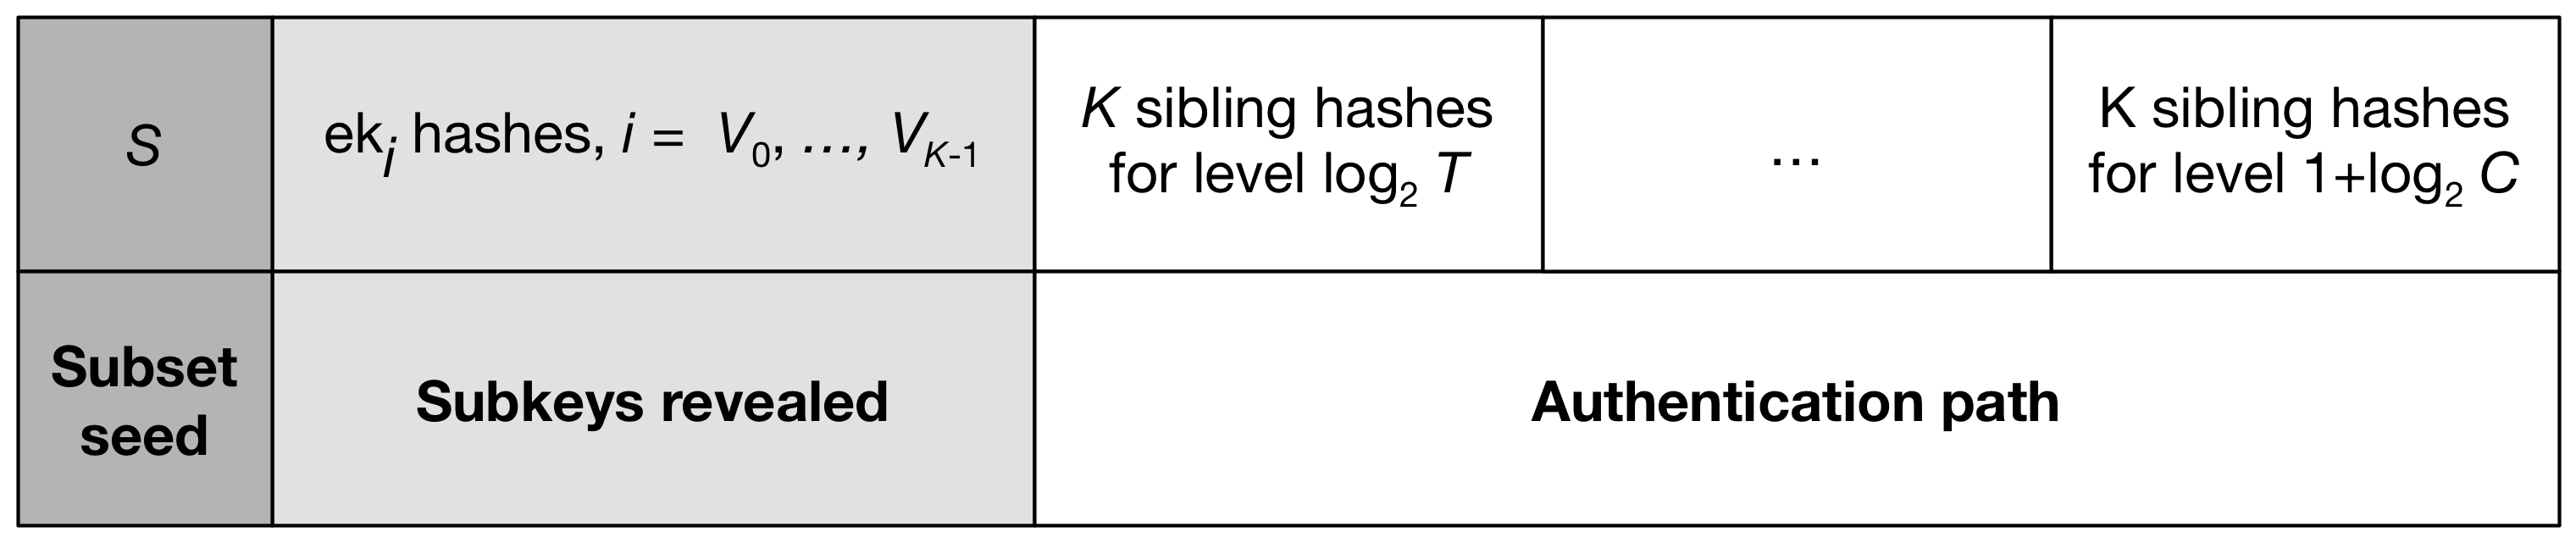
\includegraphics[width=16cm]{sig}
\caption{Content of a signature.}
\end{figure}

\section{Verifying a Signature}

Given a public key \pk and a message $M$, \gravity verifies a signature $\sig$ as follows:

\begin{enumerate}

\item Generate a subset of indices $V_0, V_1,\dots,V_{K-1}$ as per \S\ref{sec:subsetgen}, using the first 32 bytes of \sig as a signature seed.

\item For each of the $K$ indices:
\begin{enumerate}

\item Retrieve the subkey from the signature, where the subkey of index $V_i$ is the $i$th 32-byte string in the signature.

\item Using the authentication path in the signature (every other $K$ hash after the signature seed), compute parent nodes up to level $\log C$.

\item Check if the subtree root found at level $\log C$ is the same as in the public key.

\end{enumerate}
\item Verification of $\sig$ is successful only and only if all $K$ verifications succeeded.
\end{enumerate}

Step 1 requires one call to $\hashx$ and one call to $\hashz$, and at least $4K$ bytes from \drbg; step 2 requires $K$ calls to $\hashy$ and $K (\log T- \log C)$ calls to $\hashz$.


\begin{figure}
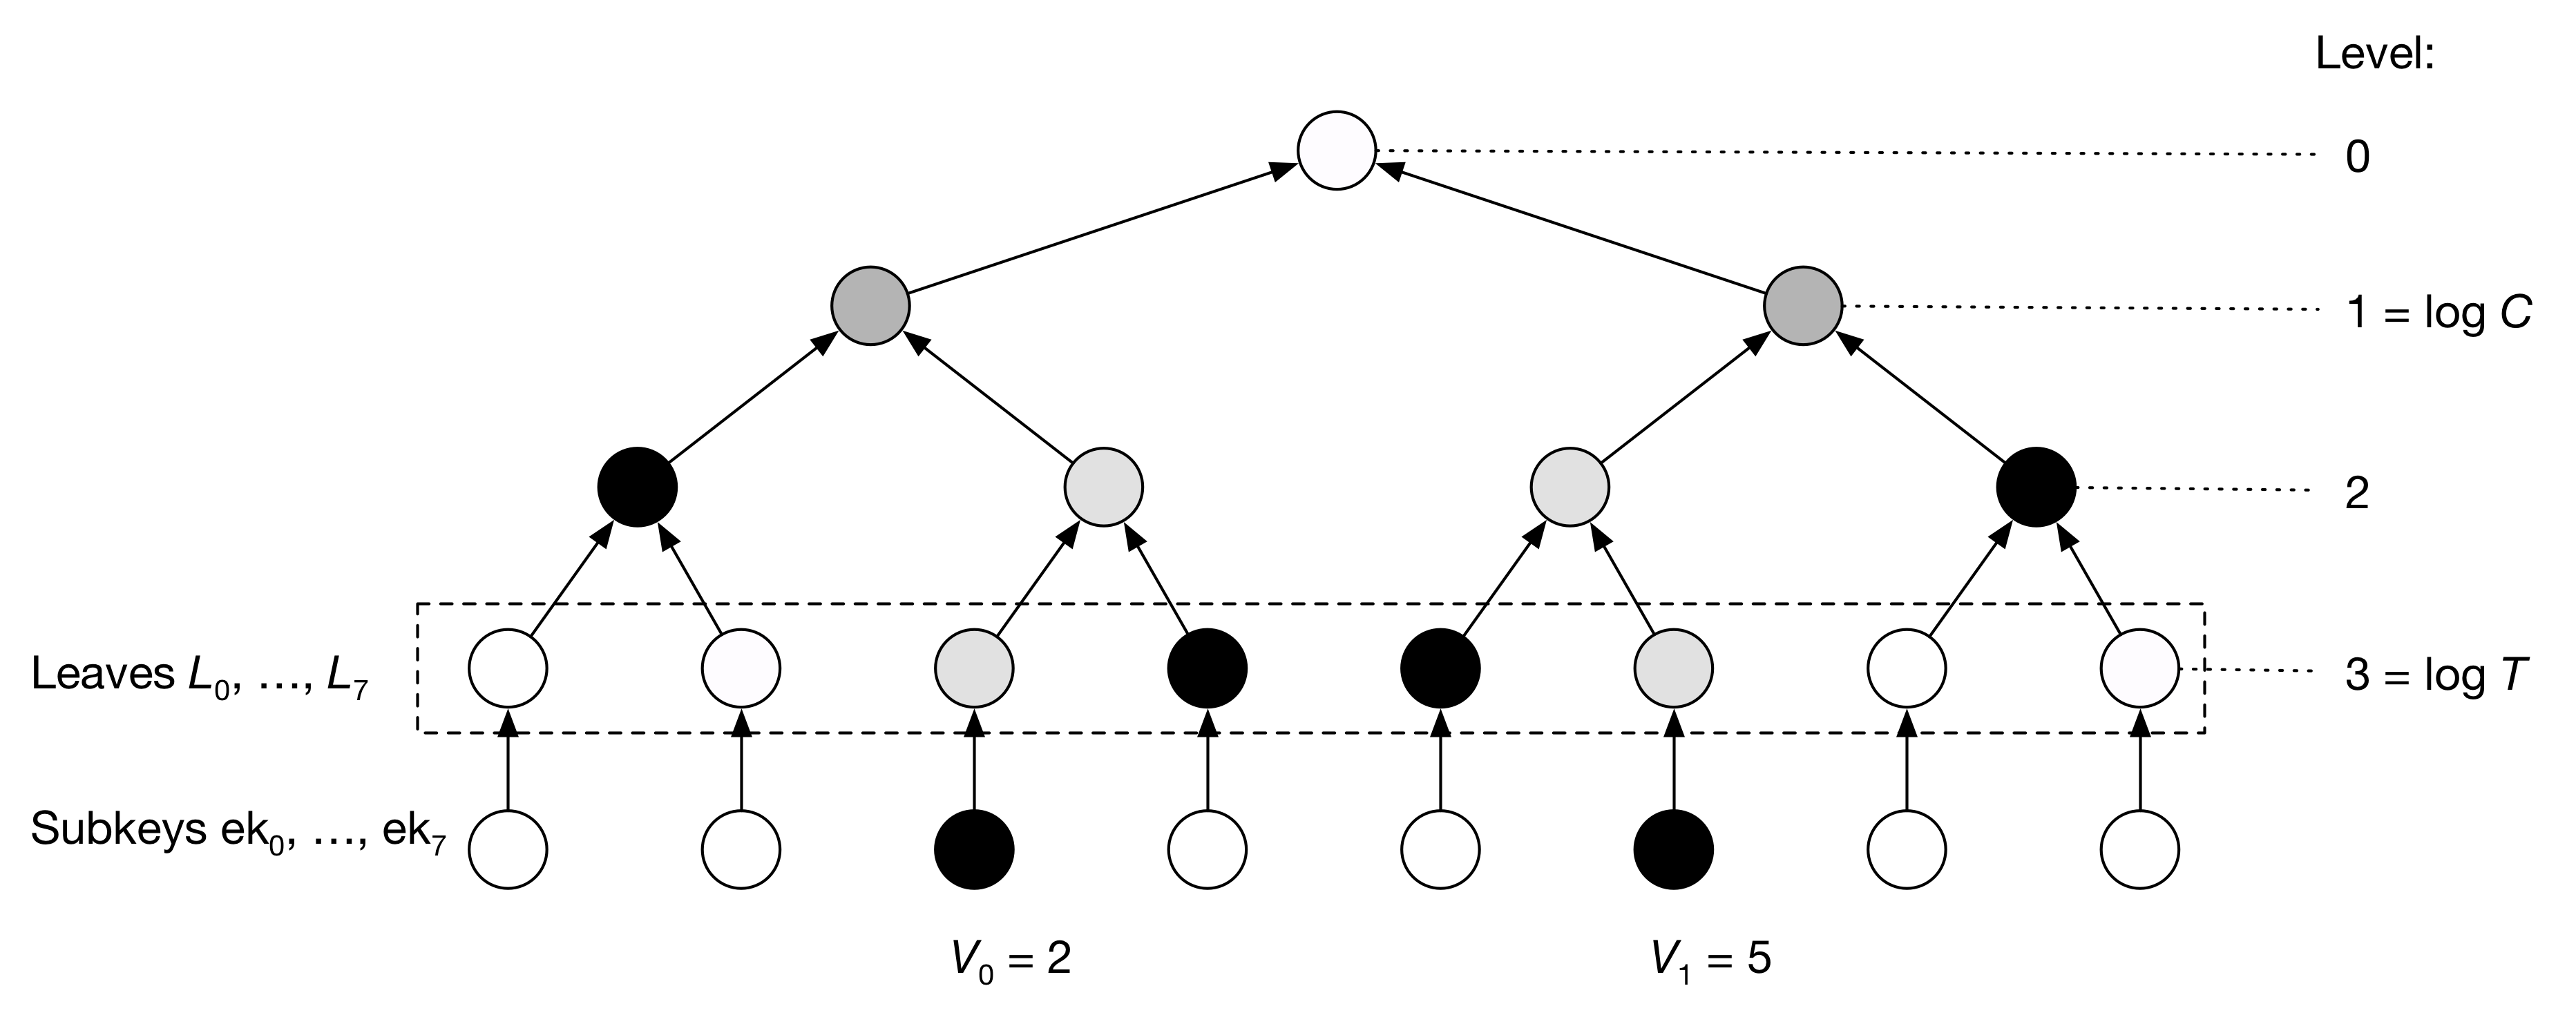
\includegraphics[width=16cm]{tree}
\caption{Binary hash tree of a signature, with a set of $T=8$ hashes (thus a tree depth of $\log T=3$), a subset of $K=2$ hashes, $C=2$ subtrees (thus their two respective roots in the public key), and subset of indexes $V_0=2, V_1=5$. The nodes in black are part of the signature, the nodes in pale grey are computed during the verification, and the nodes in dark grey are part of the public key.
}
\end{figure}

\section{Proposed Instances}

See Table~\ref{tab:instances}.

\begin{table}
\centering 
\begin{tabular}{c|ccc|c|ccc}
\toprule
\multirow{2}{*}{ID} & \multicolumn{3}{c|}{Parameters} & Messages & \multicolumn{3}{c}{Byte length} \\
& $T$ & $K$ & $C$ & limit & Sig & Pub & Priv \\
\midrule
S & $2^{17}$ & 54 & $2^{6}$ & 100 & $\num{20768}$ & 2048 & 64 \\
M & $2^{18}$ & 62 & $2^{7}$ & 300 & $\num{23840}$ & 4096 & 64 \\
L & $2^{19}$ & 64 & $2^{7}$ & 600 & $\num{26656}$ & 4096 & 64 \\
\bottomrule
\end{tabular}
\caption{Proposed \gravity instances, expected to provide 128-bit pre- and post-quantum security.}
\label{tab:instances}
\end{table}

\chapter{Security}\label{chap:security}

\section{Expected Strength}

Non-repudiation and unforgeability can be broken by finding any SHA-256 collision, since messages are SHA-256-hashed before being signed.
\gravity may also be broken if \hashx and \hashy are not collision resistant.
This puts \gravity in NIST's security category 2: ``Any attack that breaks the relevant security definition must require computational resources comparable to or greater than those required for collision search on a 256-bit hash function (e.g. SHA256/ SHA3-256)''.

Attacks that would break \gravity by searching for a subset of known subkeys fall into NIST's category 5, however: ``Any attack that breaks the relevant security definition must require computational resources comparable to or greater than those required for key search on a block cipher with a 256-bit key (e.g. AES 256)''.

Below we detail the later type of attacks.

\section{Known Attacks}\label{sec:attacks}

The main attack on \gravity works as follows:
\begin{enumerate}

    \item Observe $N$ signatures in order to collect at most $N\times K$ subkeys, and on average $(T^{NK} - (T-1)^{NK}) / T^{NK-1}$. Call the corresponding subset of indices $\mathcal{I}$.
    \item Search for a message $M$ and a signature seed $S$ such that the $K$ indices obtained by subset generation belong to $\mathcal I$, which happens with probability $(\vert\mathcal{I}\vert / T)^K$.
    \item Once a pair $(M,S)$ is found at step 2, construct the signature using the subkeys collected in step 1. The signature will be valid even though the signature seed was not derived from the secret key.
\end{enumerate}

Classically, the expected number of attempts before forging a signature is therefore
\[
\left(\frac{T}{\vert \mathcal I\vert}\right)^K = \frac{T^{NK^2}}{(T^{NK} - (T-1)^{NK})^K}
\]
where each attempt involves approximately $K/2$ AES calls in order to generate $K$ indices (since a 16-byte blocks provides at most 4 indices).

The classical security level against this attack is therefore, in bits:
\[
NK^2 \log T - K \log(T^{NK} - (T-1)^{NK}) + \log K - 2
\]
where $N$ is the number of messages signed.

A quantum attack using Grover's algorithm would require quadratically fewer attempts (approximately, and using a quantum circuit), thus a lower bound is
\[
(NK^2 \log T - K \log(T^{NK} - (T-1)^{NK}))/2 + \log K - 2
\]

For \gravity instances in Table~\ref{tab:instances}, with $N$ set to the defined message limit, instances S, M, L respectively have
\begin{itemize}
    \item Classical security levels 243.76, 253.82, 248.72
    \item Quantum security bounds 123.86, 128.79, 126.36
\end{itemize}
Figure~\ref{fig:security} shows the degradation of security as the number of signatures grows.
 

\begin{figure}
%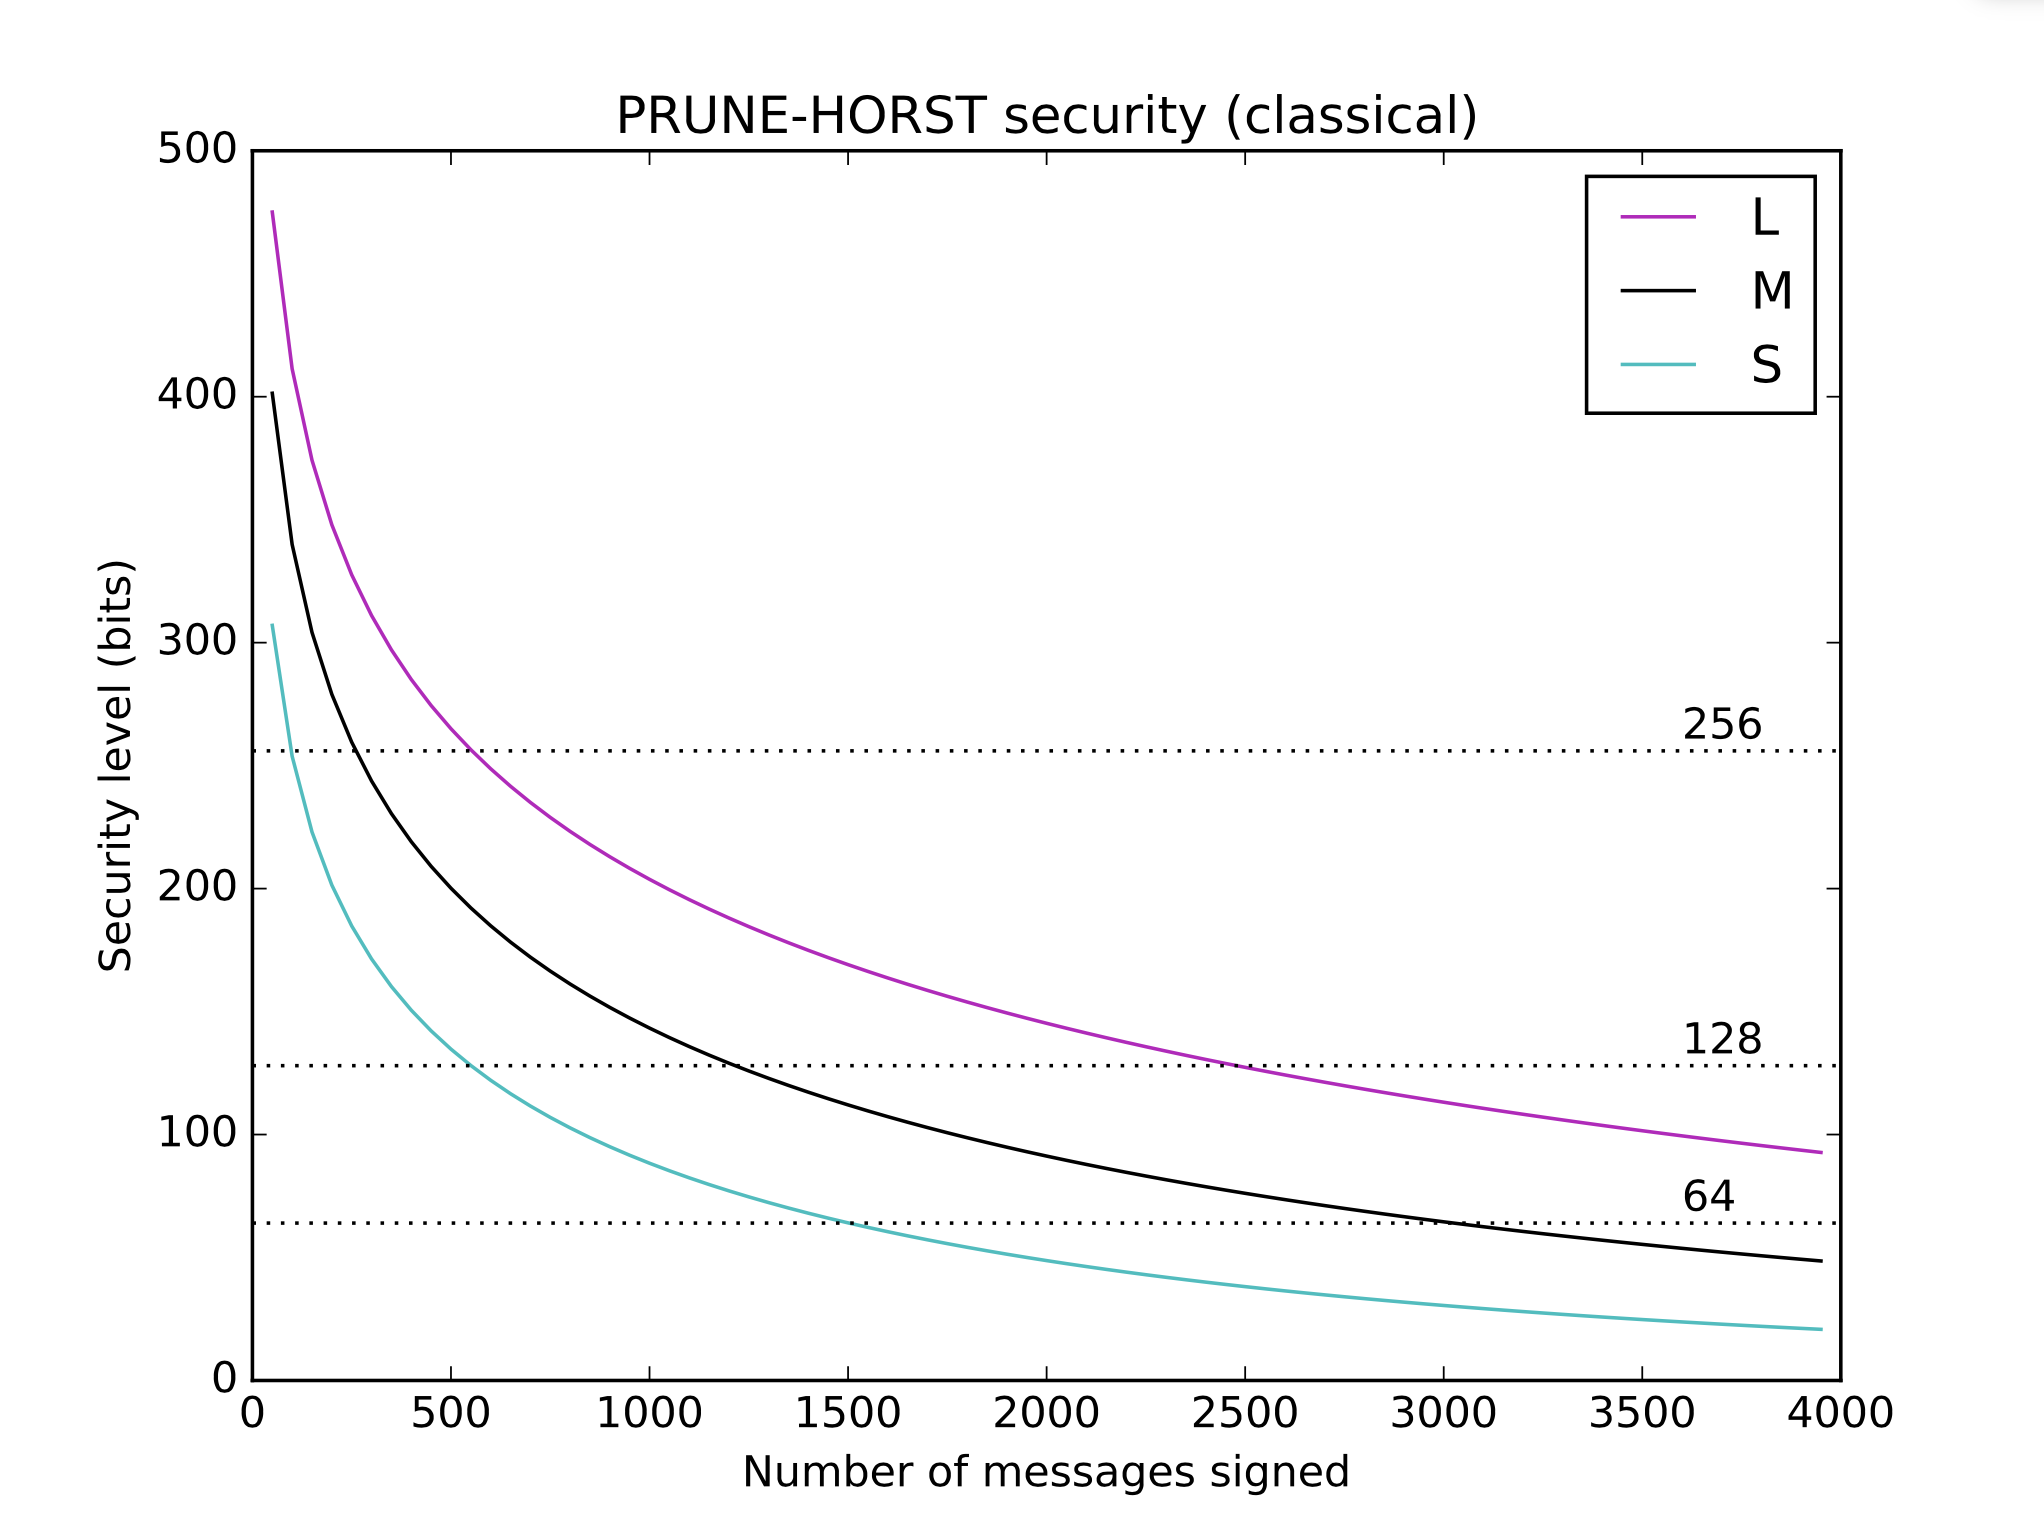
\includegraphics[width=14cm]{graph_classical}
%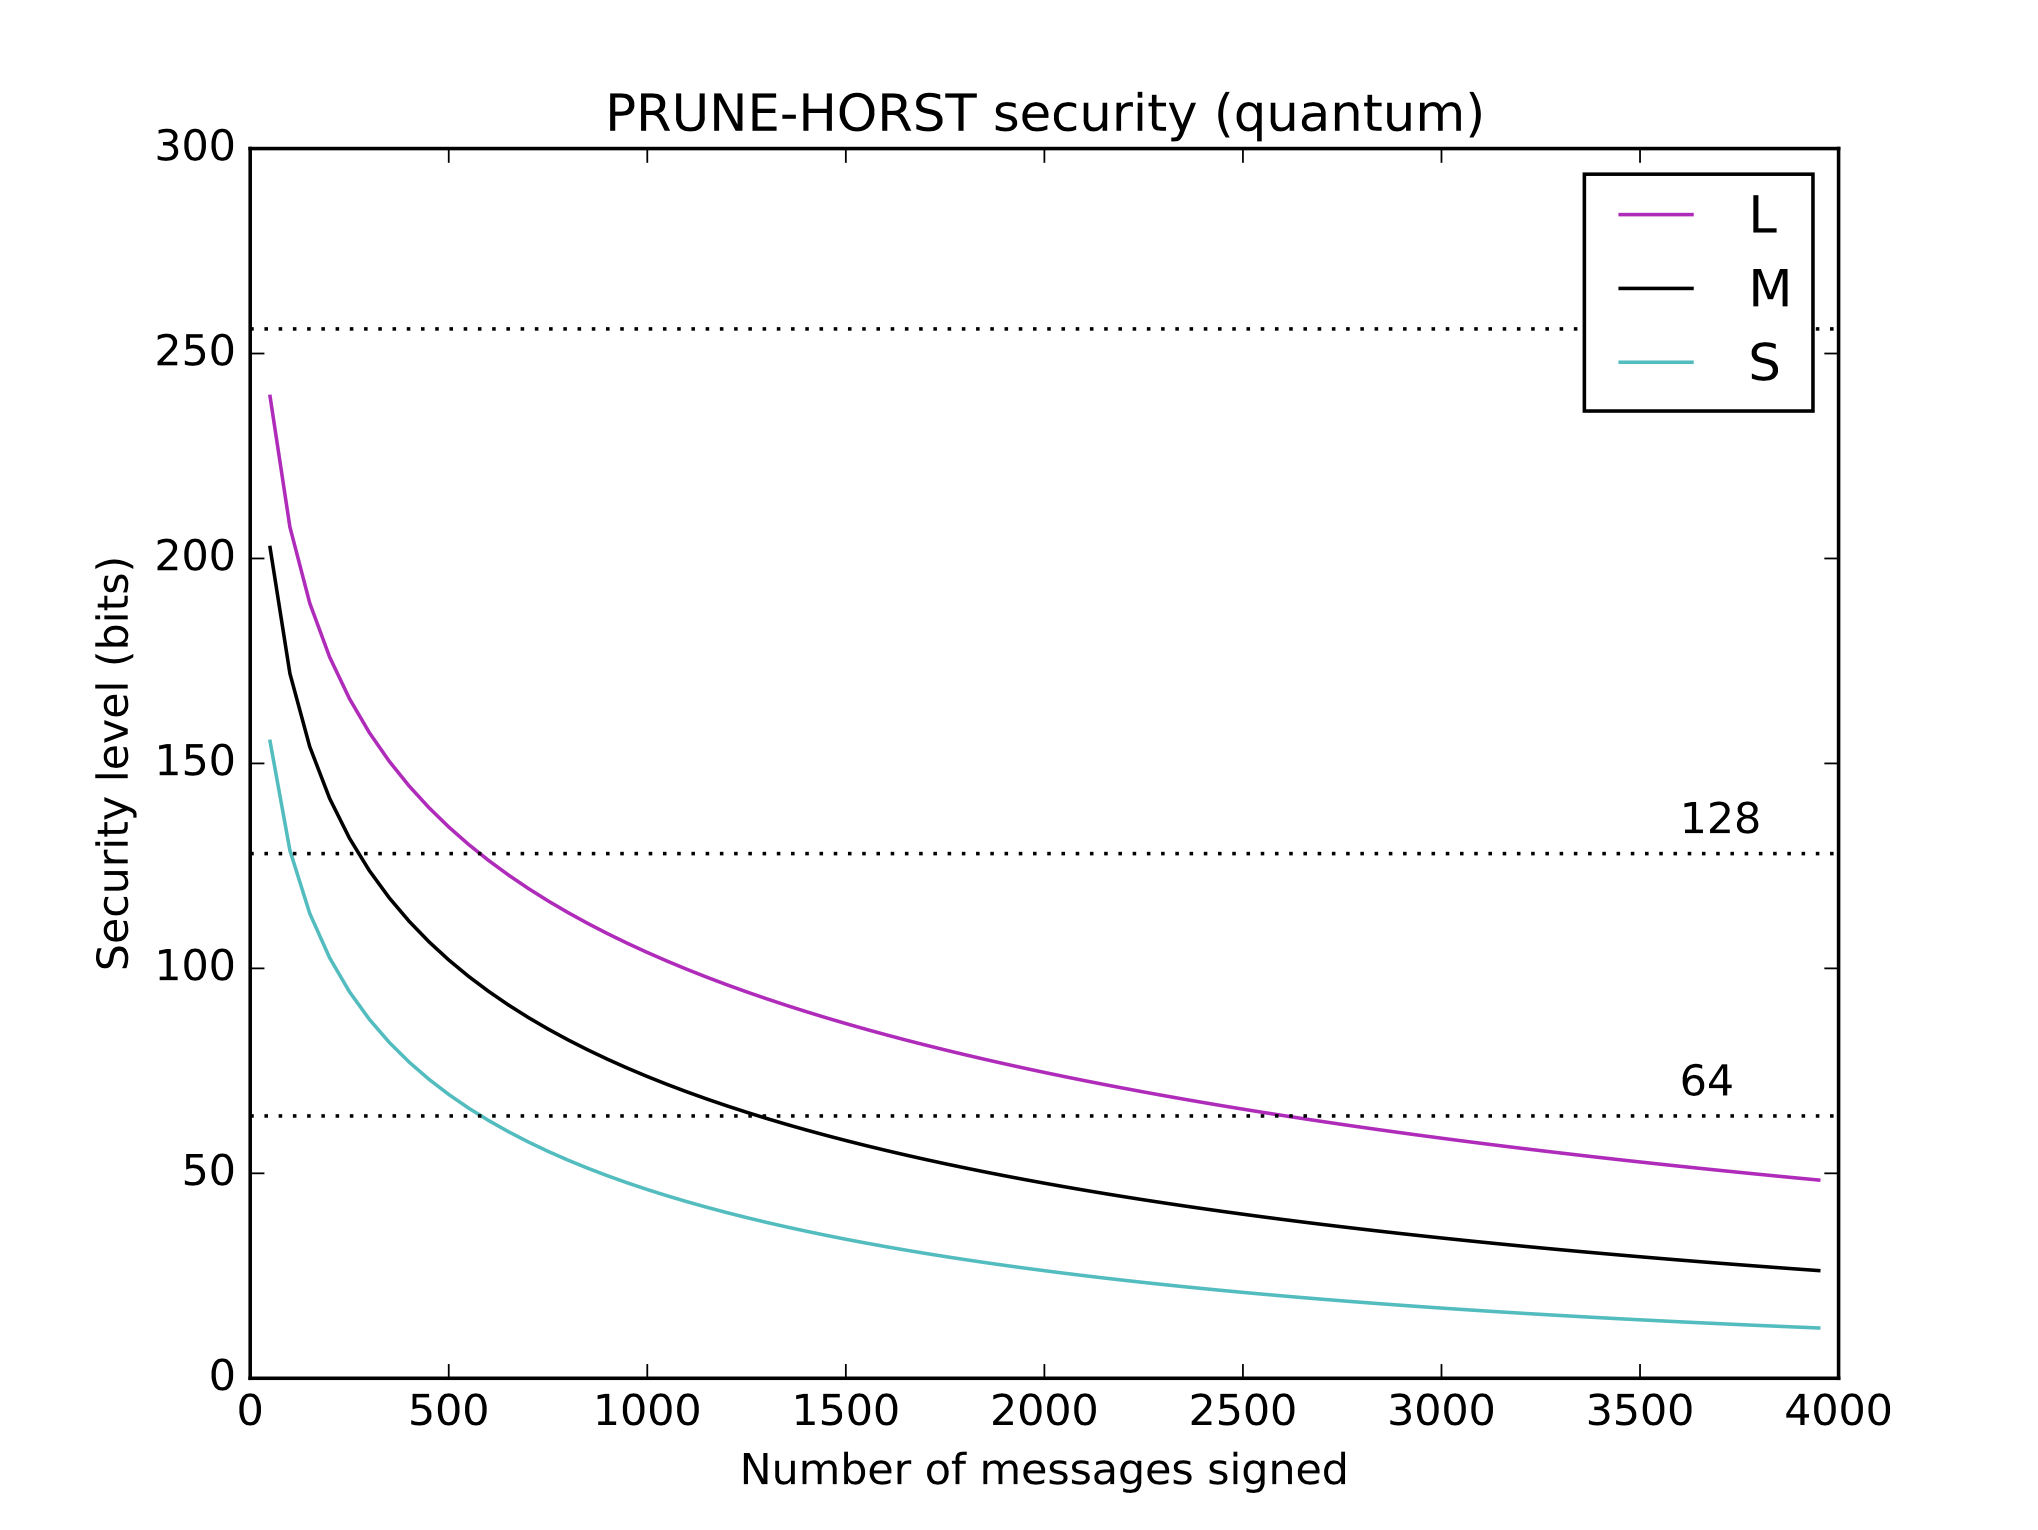
\includegraphics[width=14cm]{graph_quantum}
\centering
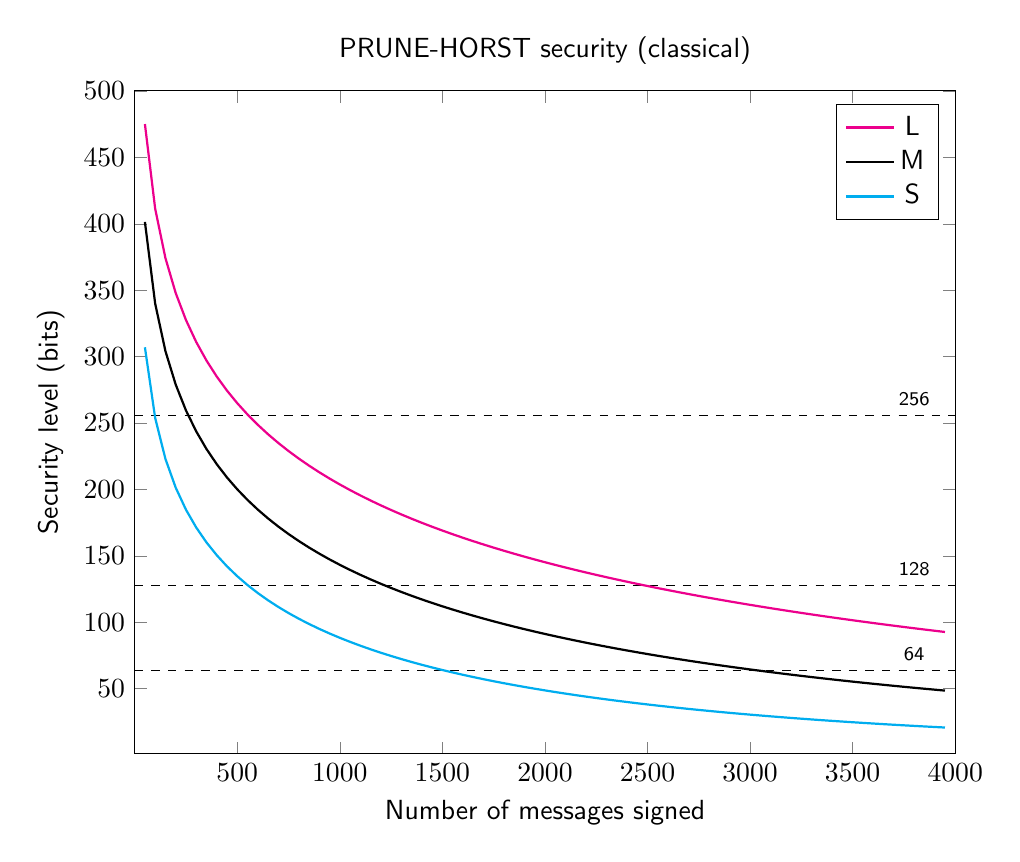
\begin{tikzpicture}
  \begin{axis}[title=PRUNE-HORST security (classical),
    width=12cm,
    height=10cm,
    xlabel=Number of messages signed,
    ylabel=Security level (bits),
    ytick distance=50,
    xtick distance=500,
    xmin=1,
    xmax=4000,
    ymin=1,
    ymax=500,
    x tick label style={
      /pgf/number format/.cd,
      set thousands separator={}
    }
  ]

\addplot[dashed,domain=1:4000,forget plot] {64};
\node[above] at (axis cs:3800,64){\scriptsize 64};

\addplot[dashed,domain=1:4000,forget plot] {128};
\node[above] at (axis cs:3800,128){\scriptsize 128};

\addplot[dashed,domain=1:4000,forget plot] {256};
\node[above] at (axis cs:3800,256){\scriptsize 256};
\addplot[magenta,thick] table {
x y
50 475.074749
100 411.356096
150 374.199556
200 347.917929
250 327.595018
300 311.041016
350 297.087815
400 285.038157
450 274.442297
500 264.993153
550 256.471694
600 248.716198
650 241.603851
700 235.039185
750 228.946523
800 223.264855
850 217.944281
900 212.943465
950 208.227779
1000 203.767930
1050 199.538915
1100 195.519222
1150 191.690210
1200 188.035618
1250 184.541179
1300 181.194303
1350 177.983829
1400 174.899812
1450 171.933355
1500 169.076466
1550 166.321939
1600 163.663256
1650 161.094500
1700 158.610282
1750 156.205686
1800 153.876208
1850 151.617716
1900 149.426407
1950 147.298777
2000 145.231587
2050 143.221836
2100 141.266743
2150 139.363722
2200 137.510365
2250 135.704428
2300 133.943812
2350 132.226556
2400 130.550823
2450 128.914888
2500 127.317132
2550 125.756030
2600 124.230149
2650 122.738136
2700 121.278713
2750 119.850676
2800 118.452881
2850 117.084248
2900 115.743754
2950 114.430427
3000 113.143343
3050 111.881626
3100 110.644441
3150 109.430995
3200 108.240530
3250 107.072326
3300 105.925694
3350 104.799977
3400 103.694547
3450 102.608802
3500 101.542169
3550 100.494097
3600 99.464060
3650 98.451551
3700 97.456086
3750 96.477201
3800 95.514448
3850 94.567398
3900 93.635639
3950 92.718775
};
\addlegendentry{L};

\addplot[black,thick] table {
x y
50 401.403132
100 339.930450
150 304.189051
200 278.981960
250 259.546610
300 243.761626
350 230.495403
400 219.072473
450 209.057146
500 200.151936
550 192.144657
600 184.878641
650 178.234910
700 172.120983
750 166.463546
800 161.203497
850 156.292495
900 151.690494
950 147.363952
1000 143.284489
1050 139.427885
1100 135.773299
1150 132.302674
1200 129.000258
1250 125.852228
1300 122.846391
1350 119.971932
1400 117.219219
1450 114.579632
1500 112.045431
1550 109.609635
1600 107.265928
1650 105.008580
1700 102.832373
1750 100.732541
1800 98.704723
1850 96.744917
1900 94.849440
1950 93.014896
2000 91.238149
2050 89.516292
2100 87.846632
2150 86.226663
2200 84.654054
2250 83.126631
2300 81.642362
2350 80.199348
2400 78.795809
2450 77.430075
2500 76.100578
2550 74.805842
2600 73.544479
2650 72.315178
2700 71.116704
2750 69.947888
2800 68.807625
2850 67.694870
2900 66.608631
2950 65.547967
3000 64.511985
3050 63.499836
3100 62.510713
3150 61.543847
3200 60.598506
3250 59.673993
3300 58.769641
3350 57.884814
3400 57.018904
3450 56.171331
3500 55.341539
3550 54.528996
3600 53.733192
3650 52.953638
3700 52.189866
3750 51.441426
3800 50.707887
3850 49.988833
3900 49.283867
3950 48.592604
};
\addlegendentry{M};

\addplot[cyan,thick] table {
x y
50 307.023459
100 253.821732
150 223.029275
200 201.410015
250 184.815908
300 171.399307
350 160.174620
400 150.553538
450 142.156589
500 134.724673
550 128.072985
600 122.065071
650 116.597309
700 111.589151
750 106.976744
800 102.708614
850 98.742658
900 95.044001
950 91.583429
1000 88.336227
1050 85.281302
1100 82.400504
1150 79.678108
1200 77.100396
1250 74.655334
1300 72.332301
1350 70.121882
1400 68.015691
1450 66.006222
1500 64.086737
1550 62.251159
1600 60.493990
1650 58.810242
1700 57.195373
1750 55.645238
1800 54.156039
1850 52.724296
1900 51.346804
1950 50.020609
2000 48.742983
2050 47.511399
2100 46.323514
2150 45.177151
2200 44.070284
2250 43.001022
2300 41.967601
2350 40.968371
2400 40.001785
2450 39.066395
2500 38.160839
2550 37.283837
2600 36.434183
2650 35.610742
2700 34.812442
2750 34.038271
2800 33.287272
2850 32.558538
2900 31.851211
2950 31.164477
3000 30.497564
3050 29.849738
3100 29.220301
3150 28.608590
3200 28.013972
3250 27.435845
3300 26.873635
3350 26.326795
3400 25.794800
3450 25.277150
3500 24.773368
3550 24.282997
3600 23.805598
3650 23.340751
3700 22.888057
3750 22.447128
3800 22.017595
3850 21.599104
3900 21.191314
3950 20.793897
};
\addlegendentry{S};


  \end{axis}
\end{tikzpicture}


\centering
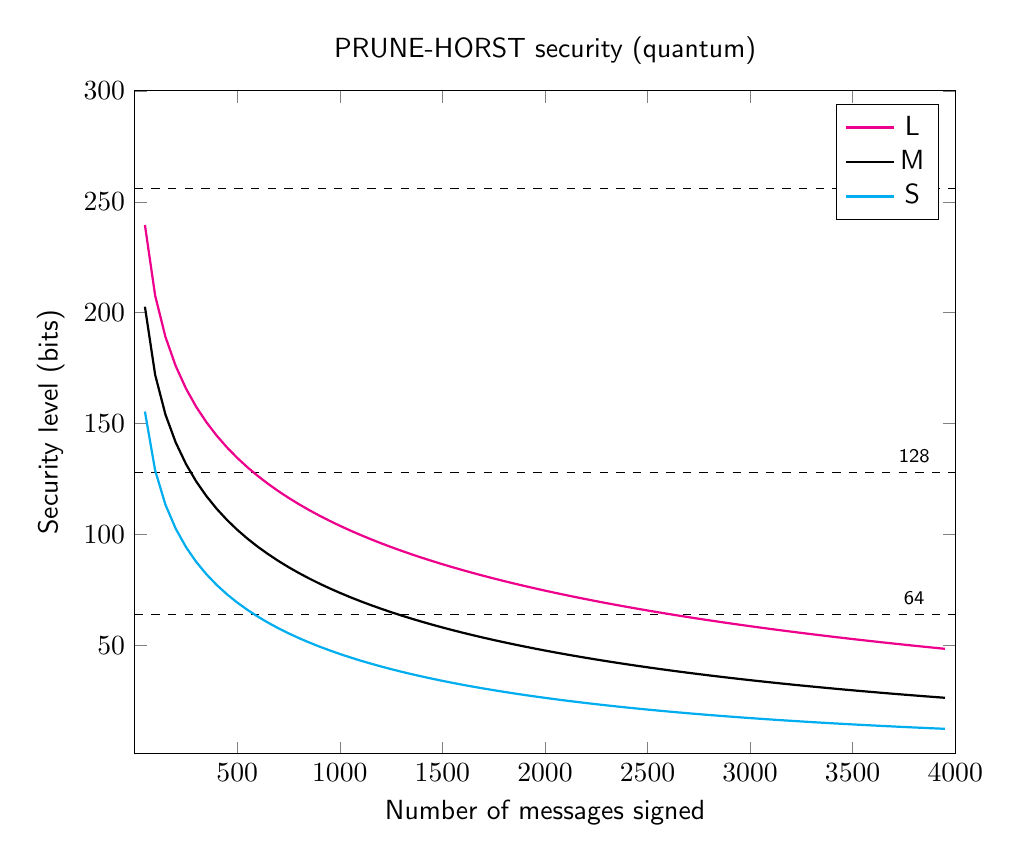
\begin{tikzpicture}
  \begin{axis}[title=PRUNE-HORST security (quantum),
    width=12cm,
    height=10cm,
    xlabel=Number of messages signed,
    ylabel=Security level (bits),
    ytick distance=50,
    xtick distance=500,
    xmin=1,
    xmax=4000,
    ymin=1,
    ymax=300,
    x tick label style={
      /pgf/number format/.cd,
      set thousands separator={}
    }
  ]

\addplot[dashed,domain=1:4000,forget plot] {64};
\node[above] at (axis cs:3800,64){\scriptsize 64};

\addplot[dashed,domain=1:4000,forget plot] {128};
\node[above] at (axis cs:3800,128){\scriptsize 128};

\addplot[dashed,domain=1:4000,forget plot] {256};
\node[above] at (axis cs:3800,256){\scriptsize 256};
\addplot[magenta,thick] table {
x y
50 239.537375
100 207.678048
150 189.099778
200 175.958965
250 165.797509
300 157.520508
350 150.543907
400 144.519078
450 139.221148
500 134.496576
550 130.235847
600 126.358099
650 122.801925
700 119.519592
750 116.473261
800 113.632428
850 110.972141
900 108.471732
950 106.113889
1000 103.883965
1050 101.769458
1100 99.759611
1150 97.845105
1200 96.017809
1250 94.270589
1300 92.597152
1350 90.991915
1400 89.449906
1450 87.966677
1500 86.538233
1550 85.160970
1600 83.831628
1650 82.547250
1700 81.305141
1750 80.102843
1800 78.938104
1850 77.808858
1900 76.713204
1950 75.649389
2000 74.615793
2050 73.610918
2100 72.633372
2150 71.681861
2200 70.755183
2250 69.852214
2300 68.971906
2350 68.113278
2400 67.275412
2450 66.457444
2500 65.658566
2550 64.878015
2600 64.115075
2650 63.369068
2700 62.639357
2750 61.925338
2800 61.226440
2850 60.542124
2900 59.871877
2950 59.215213
3000 58.571671
3050 57.940813
3100 57.322221
3150 56.715497
3200 56.120265
3250 55.536163
3300 54.962847
3350 54.399989
3400 53.847273
3450 53.304401
3500 52.771085
3550 52.247049
3600 51.732030
3650 51.225775
3700 50.728043
3750 50.238600
3800 49.757224
3850 49.283699
3900 48.817820
3950 48.359387
};
\addlegendentry{L};

\addplot[black,thick] table {
x y
50 202.678664
100 171.942323
150 154.071624
200 141.468078
250 131.750403
300 123.857911
350 117.224800
400 111.513335
450 106.505671
500 102.053066
550 98.049427
600 94.416419
650 91.094553
700 88.037590
750 85.208871
800 82.578847
850 80.123346
900 77.822345
950 75.659074
1000 73.619343
1050 71.691041
1100 69.863748
1150 68.128435
1200 66.477227
1250 64.903212
1300 63.400294
1350 61.963064
1400 60.586708
1450 59.266914
1500 57.999814
1550 56.781915
1600 55.610062
1650 54.481388
1700 53.393285
1750 52.343369
1800 51.329460
1850 50.349557
1900 49.401818
1950 48.484546
2000 47.596172
2050 46.735244
2100 45.900414
2150 45.090430
2200 44.304125
2250 43.540414
2300 42.798279
2350 42.076772
2400 41.375003
2450 40.692136
2500 40.027387
2550 39.380019
2600 38.749337
2650 38.134687
2700 37.535450
2750 36.951042
2800 36.380911
2850 35.824533
2900 35.281414
2950 34.751082
3000 34.233091
3050 33.727016
3100 33.232455
3150 32.749022
3200 32.276351
3250 31.814095
3300 31.361918
3350 30.919505
3400 30.486550
3450 30.062764
3500 29.647868
3550 29.241596
3600 28.843694
3650 28.453917
3700 28.072031
3750 27.697811
3800 27.331042
3850 26.971515
3900 26.619032
3950 26.273400
};
\addlegendentry{M};

\addplot[cyan,thick] table {
x y
50 155.389173
100 128.788310
150 113.392081
200 102.582451
250 94.285398
300 87.577097
350 81.964754
400 77.154213
450 72.955738
500 69.239780
550 65.913936
600 62.909979
650 60.176098
700 57.672019
750 55.365816
800 53.231751
850 51.248773
900 49.399444
950 47.669158
1000 46.045557
1050 44.518095
1100 43.077696
1150 41.716498
1200 40.427642
1250 39.205111
1300 38.043594
1350 36.938385
1400 35.885289
1450 34.880555
1500 33.920812
1550 33.003023
1600 32.124439
1650 31.282565
1700 30.475130
1750 29.700063
1800 28.955463
1850 28.239592
1900 27.550846
1950 26.887748
2000 26.248935
2050 25.633143
2100 25.039201
2150 24.466019
2200 23.912586
2250 23.377955
2300 22.861244
2350 22.361629
2400 21.878336
2450 21.410641
2500 20.957863
2550 20.519362
2600 20.094535
2650 19.682815
2700 19.283665
2750 18.896579
2800 18.521080
2850 18.156713
2900 17.803049
2950 17.459682
3000 17.126226
3050 16.802313
3100 16.487594
3150 16.181739
3200 15.884430
3250 15.595366
3300 15.314261
3350 15.040841
3400 14.774844
3450 14.516019
3500 14.264128
3550 14.018942
3600 13.780243
3650 13.547819
3700 13.321472
3750 13.101008
3800 12.886241
3850 12.676996
3900 12.473101
3950 12.274392
};
\addlegendentry{S};


  \end{axis}
\end{tikzpicture}


\caption{Security level in bits of \gravity instances against classical and quantum attacks exploiting the subkeys revealed in previous signatures. Quantum attacks use Grover search to get a quadratic speed-up over classical attacks.}
\label{fig:security}
\end{figure}

\section{Other Attacks}

Fault attacks or side-channel attacks could recover $\sk_1$ in the subset generation if the AES implementation is not protected.
Likewise $\sk_2$ could be recovered during the computation of $S=\hashz(\sk_2 \Vert \hashx(M))$ if $\hashz$ is not protected.

Fault attacks could also force subset generation to return indices of specific subkeys.

Timing attacks are unlikely if the implementations of functions processing $\sk_1$ and $\sk_2$ are time-constant (AES, Haraka-v2).


\section{Forgery Detection}\label{sec:detection}

In the attack described in \S\ref{sec:attacks} the attacker chooses the signature seed $S$ but can't pick $S=\hashz(\sk_2 \Vert \hashx(M))$, as prescribed by the signing procedure.
Yet the signature will be verified, and only the legitimate signer can determine that $S$ wasn't properly chosen using $\sk_2$.
EdDSA (and Ed25519) have a similar property of invalid-yet-valid signatures.

This property allows a signer to detect signatures forged after exploiting a (too) high number of issued signatures, compared with legitimately computed signatures.
But it can't be used to prove the existence of forgeries to a third-party, since the signer could have themselves used an invalid signature seed in order to break non-repudiation.
If the signer is trusted, however, then they can reveal $\sk_2$ privately in order to show evidence of a forgery.
\chapter{Performance}\label{chap:performance}

\section{Complexity}

Most of operations in \gravity are AES rounds, through AES-256-CTR, Haraka-256, or Haraka-512. 
AES-256-CTR does 14 AES rounds per 16-byte block generated.
Haraka-256 does 24 AES rounds per 32-byte value hashed, and Haraka-512 does 48 rounds per 64-byte value hashed.
% TODO: check these 24 and 48

Table~\ref{tab:complexity} gives the count of these operations for each \gravity instance, where
\begin{itemize}
    \item Key generation needs $100T- 48C$ AES rounds

    \item Signature needs $100T - 48C + 7K + 96$ AES rounds, where we count $8K$ bytes for subset generation, as in our reference code (thus $K/2$ AES calls, or $7K$ rounds)
    
    \item Verification needs $K(24 + 48(\log T - \log C) + 7K + 48$ AES rounds
\end{itemize}

We ignore the cost of hashing the message with \hashx, and we also ignore the potential speed-up of pipelined or parallel computation of AES rounds.

\begin{table}
\centering 
\begin{tabular}{cc|ccc|c}
\toprule
Operation & ID & AES-256 & Haraka-256 & Haraka-512 & AES rounds \\
\midrule
\multirow{3}{*}{Key generation}
& S & $\num{262144}$ & $\num{131072}$ & $\num{131008}$ & $\num{13104128}$ \\
& M & $\num{524288}$ & $\num{262144}$ & $\num{262016}$ & $\num{26208256}$ \\
& L & $\num{1048576}$ & $\num{524288}$ & $\num{524160}$ & $\num{52422656}$ \\
\midrule
\multirow{3}{*}{Signature}
& S & $\num{262171}$ & $\num{131072}$ & $\num{131010}$ & $\num{13104602}$ \\
&M & $\num{524319}$ & $\num{262144}$ & $\num{262018}$ & $\num{26208786}$ \\
&L & $\num{1048608}$ & $\num{524288}$ & $\num{524162}$ & $\num{52423200}$ \\
\midrule
\multirow{3}{*}{Verification} 
& S & 27 & 54 & $595$ & $\num{30234}$ \\
&M & 31 & 62 & $683$ & $\num{34706}$ \\
&L & 32 & 64 & $769$ & $\num{38896}$ \\
\bottomrule
\end{tabular}

\caption{Complexity of \gravity instances, where AES-256 does 14 rounds per block, Haraka-256 does 24 AES rounds, and Haraka-512 does 48. The count of AES-256 blocks for subset generation is an upper bound.}
\label{tab:complexity}
\end{table}

Verification is orders of magnitude faster than signature generation, which is ideal for the \gravity use cases: typically few signatures would be generated on powerful machines with no speed constraint, whereas verification may be performed multiple times on less powerful machines (for example, for firmware signatures or CA-issued certificates).

\section{Choosing a Number of Subtrees}\label{sec:tradeoff}

The number of substrees $C$ does not affect the security of the scheme, but allows to reduce the signature size by increasing the public key size: instead of including only the root of the tree (case $C=1$), the public key can include all the roots of subtrees at a lower level.

A larger $C$ also makes signature and verification slightly faster.

For the \gravity instances proposed, we choose the value of $C$ that minimizes the total length signature + public key. 
Other values of $C$ may be used to reduce the signature size or speed-up computations.

Figure~\ref{fig:subtrees} shows the different trade-offs for the proposed \gravity instances.

\begin{figure}
\centering
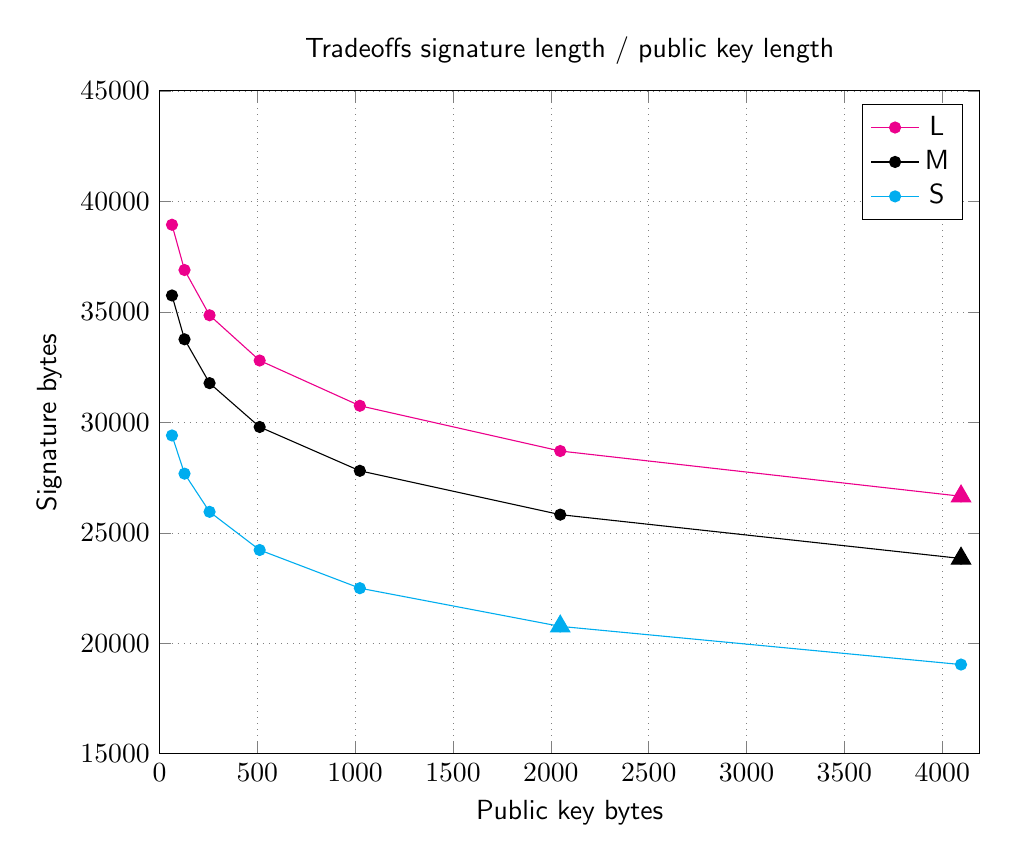
\begin{tikzpicture}
  \begin{axis}[title=Tradeoffs signature length / public key length,
    width=12cm,
    height=10cm,
    xlabel=Public key bytes,
    ylabel=Signature bytes,
    ytick distance=5000,
    xtick distance=500,
    xmin=0,
    xmax=4192,
    ymin=15000,
    ymax=45000,
    x tick label style={
      /pgf/number format/.cd,
      set thousands separator={}
    },
    scaled y ticks=false,
    y tick label style={
      /pgf/number format/.cd,
      set thousands separator={}
    },
    grid style={help lines,dotted},
    grid=major
  ]

\addplot[magenta,mark=*] coordinates {
(64, 38944.000000)
(128, 36896.000000)
(256, 34848.000000)
(512, 32800.000000)
(1024, 30752.000000)
(2048, 28704.000000)
(4096, 26656.000000)
};
\addlegendentry{L};
\addplot[black,mark=*] coordinates {
(64, 35744.000000)
(128, 33760.000000)
(256, 31776.000000)
(512, 29792.000000)
(1024, 27808.000000)
(2048, 25824.000000)
(4096, 23840.000000)
};
\addlegendentry{M};
\addplot[cyan,mark=*] coordinates {
(64, 29408.000000)
(128, 27680.000000)
(256, 25952.000000)
(512, 24224.000000)
(1024, 22496.000000)
(2048, 20768.000000)
(4096, 19040.000000)
};
\addlegendentry{S};
\addplot[only marks,mark=triangle*,mark size=4pt,magenta] coordinates {
(4096, 26656.000000)
};
\addplot[only marks,mark=triangle*,mark size=4pt,black] coordinates {
(4096, 23840.000000)
};
\addplot[only marks,mark=triangle*,mark size=4pt,cyan] coordinates {
(2048, 20768.000000)
};

  \end{axis}
\end{tikzpicture}


%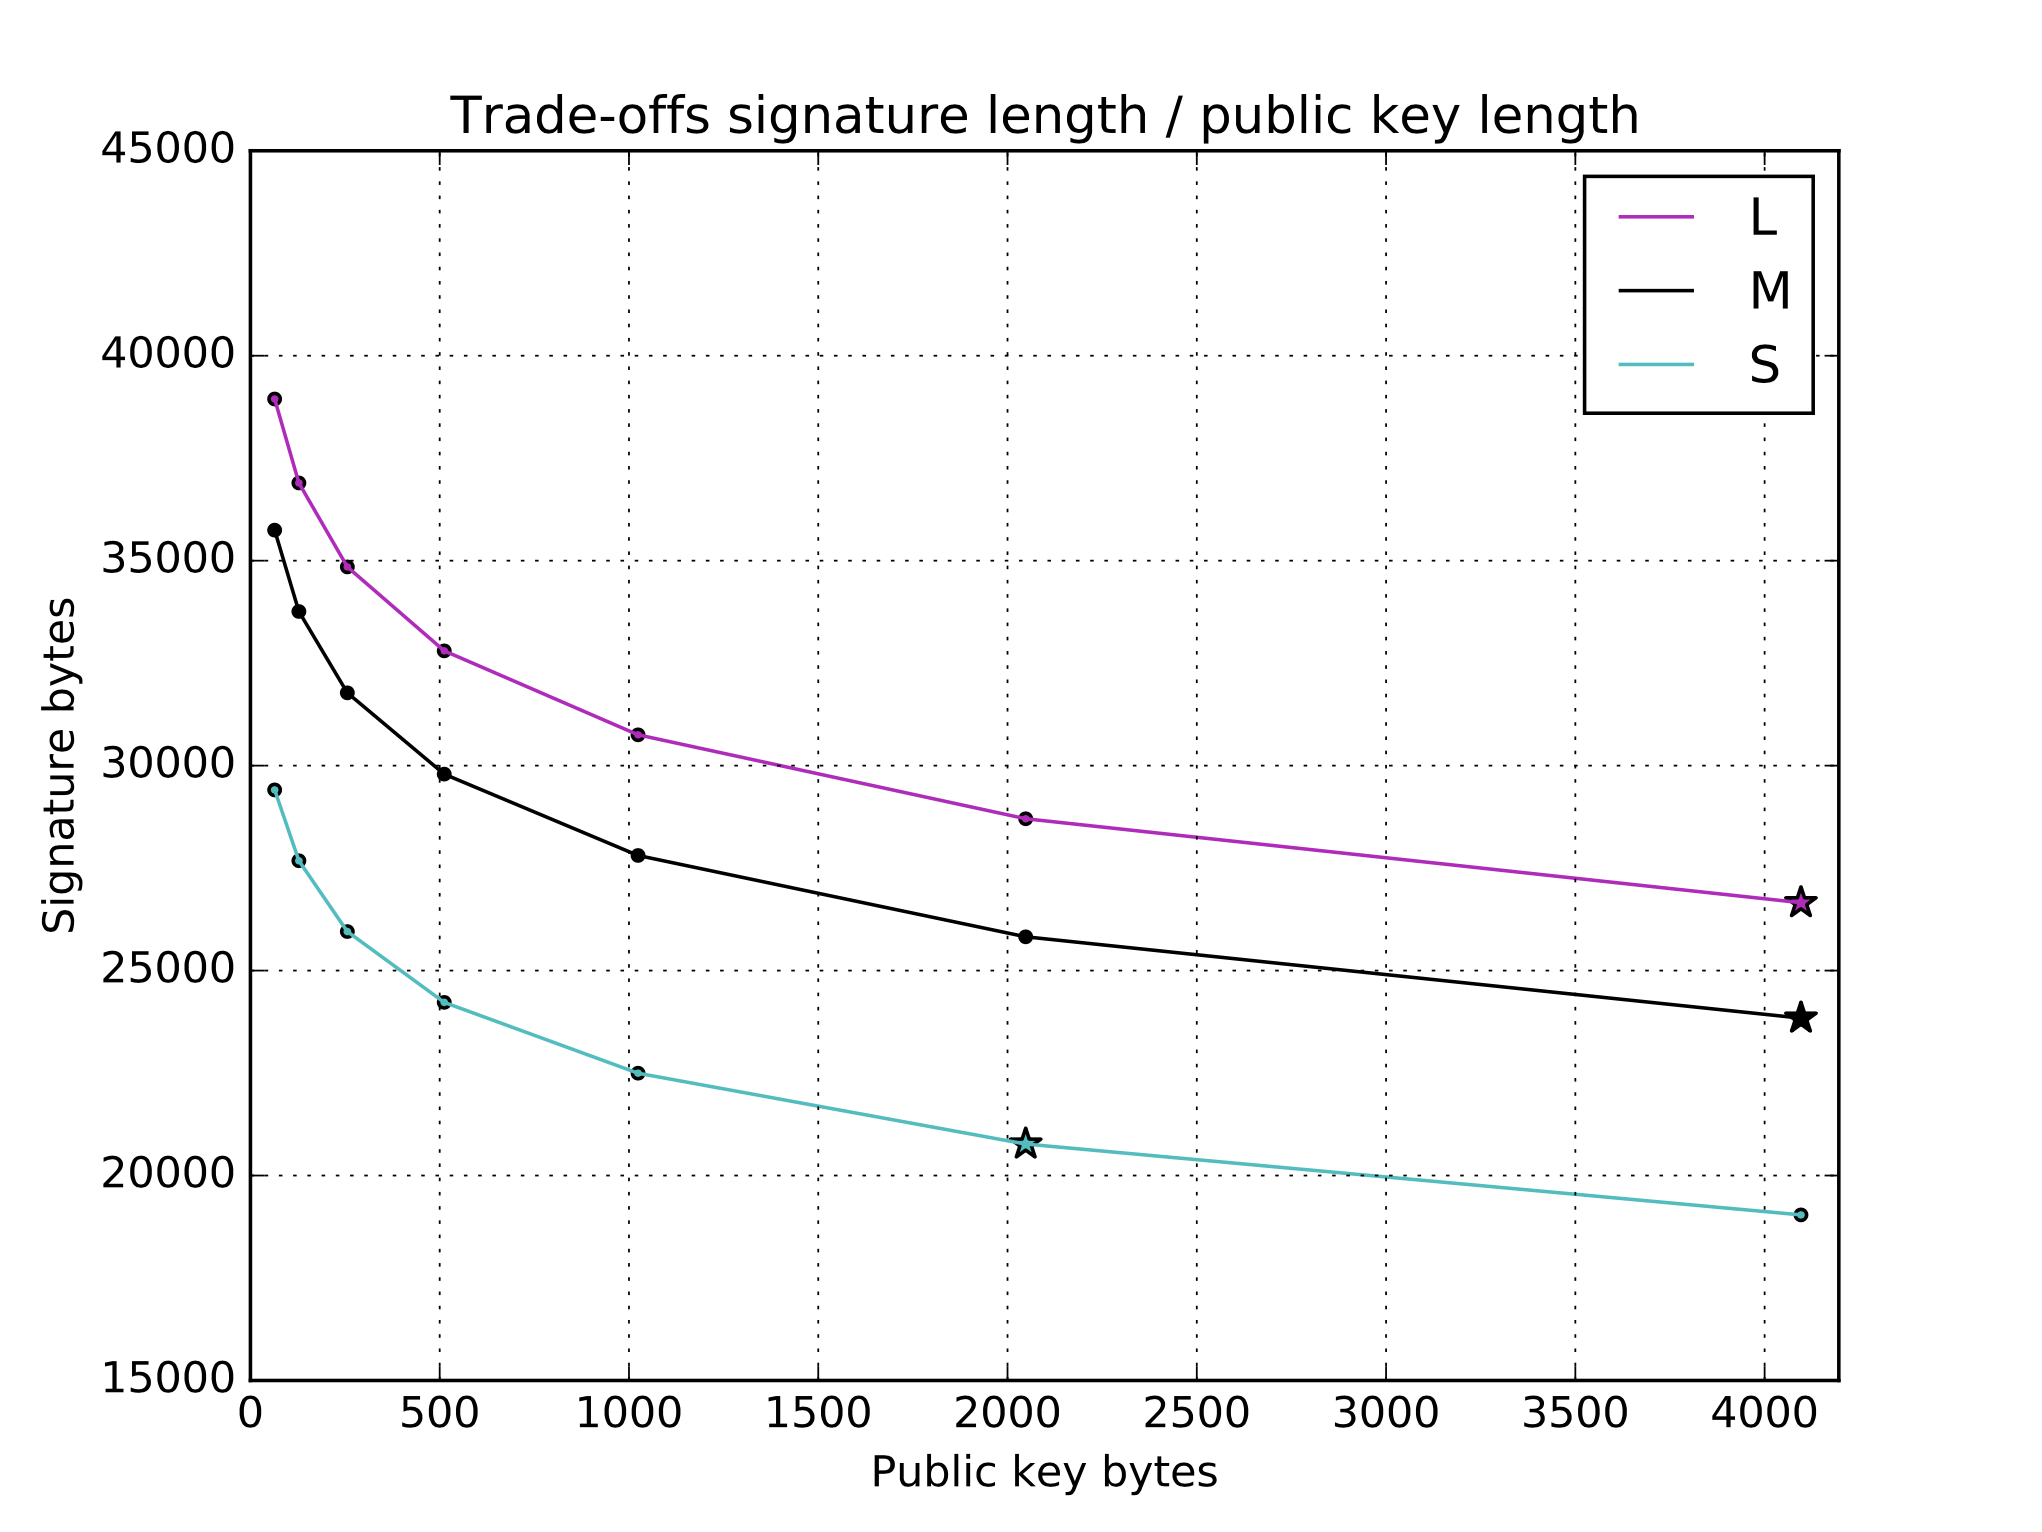
\includegraphics[width=14cm]{graph_subtrees}
\caption{Trade-offs between signature length and public-key length, for $C$ in $\{2^1, 2^2, \dots, 2^7\}$. The triangles indicate the optimal trade-offs, chosen for the instances proposed.}
\label{fig:subtrees}
\end{figure}


\section{Software Performance}

The AES rounds that constitute most of \gravity computations and the largest part of the execution time can be implemented with native AES instructions (AES-NI).

On Skylake CPUs, the AES round instruction AESENC has a latency of four cycles and a reciprocal throughput of one.
In \gravity, many AES rounds can be pipelined in order to maximize the effective throughput and return one AESENC result per cycle: Haraka-512 computes up to four independent AES rounds, and rounds within four AES-256-CTR instances can be interleaved.

These independent AES round instances can't really be parallelized on current microarchitectures that have a single AES unit. 
But AMD's new Ryzen CPUs have two AES units, and Intel is expect to follow in future microarchitectures versions and include two AES units as well.

Our optimized implementation thus includes 4-way and 8-way interleaved versions of Haraka for computing the trees and its leaves\footnote{Based on Haraka's authors code at \url{https://github.com/kste/haraka/}, with a few optimizations and bug fixes.}, as well as 4-way interleaved AES-256-CTR.

Signature verification requires only negligible memory: our implementation only allocates $140+K$ bytes on the stack, which is probably suboptimal. 

Our implementations of key generation and signing, however, allocate $32T$ heap bytes to store the subkeys and compute the tree.
This is respectively 4MiB, 8MiB, and 16MiB for instances S, M, and L.
But key generation and signing can be implemented to use much less memory, for example using techniques described in~\cite{armed}.

Below we report example results from running our benchmark program (\texttt{make bench}) on a Intel Core i7-6700 CPU @ 3.40GHz (Turbo Boost disabled), where the wall time is given in microseconds, and \texttt{crypto\_sign\_cached} implements the trick described in \S\S\ref{ssec:cache}:

Version S ($T=2^{17}, C=2^6, K=54$):
{\footnotesize
\begin{verbatim}
# crypto_sign_keypair
median cycles count:     14054574
average wall time:       4124.561 usec

# crypto_sign
median cycles count:     19551800
average wall time:       5747.488 usec

# crypto_sign_cached
median cycles count:     10418326
average wall time:       3063.229 usec

# crypto_sign_open
median cycles count:     72908
average wall time:       21.443 usec
\end{verbatim}
}

Version M ($T=2^{18}, C=2^7, K=62$):
{\footnotesize
\begin{verbatim}
# crypto_sign_keypair
median cycles count:     28193440
average wall time:       8276.869 usec

# crypto_sign
median cycles count:     40179136
average wall time:       11813.293 usec

# crypto_sign_cached
median cycles count:     20982546
average wall time:       6169.703 usec

# crypto_sign_open
median cycles count:     83650
average wall time:       24.598 usec
\end{verbatim}
}

Version L ($T=2^{19}, C=2^7, K=64$):
{\footnotesize
\begin{verbatim}

# crypto_sign_keypair
median cycles count:     58782818
average wall time:       17234.963 usec

# crypto_sign
median cycles count:     80689918
average wall time:       23750.260 usec

# crypto_sign_cached
median cycles count:     42442734
average wall time:       12473.613 usec

# crypto_sign_open
median cycles count:     93702
average wall time:       27.562 usec
\end{verbatim}
}
Note the low verification time for all instances (\texttt{crypto\_sign\_open}).


\section{Hardware Performance}

Hardware architecture may trivially parallelize AES-256 calls within AES-256-CTR, as well as Haraka instances (and AES rounds within Haraka).
Many speed/area trade-offs are therefore possible.


\section{Possible Optimizations}

\subsection{Faster Signing with Key Caching}\label{ssec:cache}

Instead of taking a 64-byte secret key and expanding it to a $32T$-byte set of subkeys for each new signature, you can compute the subkeys once and cache it for future signatures. 
This saves $2T$ calls to AES-256, or $28T$ AES rounds, or 28\% of the total AES rounds done when signing.


\subsection{32-Byte Public Keys with Octopus}

Authentication paths in a signature may contain several times the same value, if paths from two leaves merge and therefore have the same authentication paths from this point.
To avoid these redundancies and offer optimally short signatures, we analyzed this trick---called ``Octopus''--in~\cite[Ch.5]{masters}, and developed tools to compute the expected number of hashes required in an authentication path.
Indeed, the amount of redundancy depends on the choice of the $K$ indices, and therefore a signature's length will depend on the message hashed.

Since most redundancies will occur in the higher levels of the tree, Octopus can be used to create optimally short signatures while having a single subtree root in the public key ($C=1$), and therefore a 32-byte public key.

Table~\ref{tab:octopus} shows the expected length of a signature if Octopus is used, comparing with the default length of $K(\log T - \log C)+K$ hashes plus the 32-byte signature seed.
% TODO: table: ID | siglen (hashes) | mean (hashes) | stdev (hashes)

\begin{table}
\centering 
\begin{tabular}{c|cc|cc}
\toprule
\multirow{2}{*}{ID} & 
\multicolumn{2}{c|}{Default} &
\multicolumn{2}{c}{Octopus} \\

& Length & Hashes & Hashes & Length \\
\midrule
S & $\num{20768}$ & 648 & $614.03$ & $\num{19681}$ \\
M & $\num{23840}$ & 744 & $754.47$ & $\num{24143}$ \\
L & $\num{26656}$ & 832 & $839.81$ & $\num{26906}$ \\
\bottomrule
\end{tabular}
\caption{Length of a signature without and with the Octopus trick to eliminate redundancies in a signature and use a 32-byte public key. We show the signature byte length (including the signature seed), as well as the number of 32-byte hash values forming the authentication path, including the $K$ leaves, but excluding the signature seed.}
\label{tab:octopus}
\end{table}




\bibliographystyle{plainurl}
\bibliography{bib}


% \input notes %replace with todo

\end{document}
